% This must be in the first 5 lines to tell arXiv to use pdfLaTeX, which is strongly recommended.
\pdfoutput=1
% In particular, the hyperref package requires pdfLaTeX in order to break URLs across lines.

\documentclass[11pt]{article}

% Remove the "review" option to generate the final version.
\usepackage[]{ACL2023}

% Standard package includes
\usepackage{times}
\usepackage{latexsym}

% For proper rendering and hyphenation of words containing Latin characters (including in bib files)
\usepackage[T1]{fontenc}
% For Vietnamese characters
% \usepackage[T5]{fontenc}
% See https://www.latex-project.org/help/documentation/encguide.pdf for other character sets

% This assumes your files are encoded as UTF8
\usepackage[utf8]{inputenc}

% This is not strictly necessary, and may be commented out.
% However, it will improve the layout of the manuscript,
% and will typically save some space.
\usepackage{microtype}

% This is also not strictly necessary, and may be commented out.
% However, it will improve the aesthetics of text in
% the typewriter font.
\usepackage{inconsolata}

\usepackage{graphicx}
\usepackage{multirow}


% If the title and author information does not fit in the area allocated, uncomment the following
%
%\setlength\titlebox{<dim>}
%
% and set <dim> to something 5cm or larger.

\title{Do Hybrid and Abstractive Summarization Methods Improve Performance Over Extractive Summarization Methods in Legal Documents?}

% Author information can be set in various styles:
% For several authors from the same institution:
% \author{Author 1 \and ... \and Author n \\
%         Address line \\ ... \\ Address line}
% if the names do not fit well on one line use
%         Author 1 \\ {\bf Author 2} \\ ... \\ {\bf Author n} \\
% For authors from different institutions:
% \author{Author 1 \\ Address line \\  ... \\ Address line
%         \And  ... \And
%         Author n \\ Address line \\ ... \\ Address line}
% To start a seperate ``row'' of authors use \AND, as in
% \author{Author 1 \\ Address line \\  ... \\ Address line
%         \AND
%         Author 2 \\ Address line \\ ... \\ Address line \And
%         Author 3 \\ Address line \\ ... \\ Address line}

\author{Chris John, Daniel Yi, and Ryan Schaefer \\
  University of California, Berkeley \\
  Berkeley, CA, United States \\
  \texttt{\{chrisjohn47,daniel\_yi,ryan\_schaefer\}@berkeley.edu} }

\begin{document}
\maketitle
\begin{abstract}
Summarizing legislative documents can lead to distinct challenges due to their complexity, length, and structured nature. While traditional extractive methods like Cluster Extraction and MMR (Maximal Marginal Relevance) have been previously utilized due to their efficiency and interpretability, newer methods in hybrid and abstractive techniques bring a newer, potentially more promising alternative. In this paper, we aim to evaluate extractive, hybrid, and abstractive summarization methods on the BillSum dataset, a compilation of U.S. Congressional and California State bills. In specific, we explored Cluster Extraction methods combined with LED (Longformer Encoder-Decoder), as well as MMR paired with PEGASUS and BigBird PEGASUS. Our results ultimately demonstrated that hybrid methods, particularly utilizing Cluster Extraction combined with LED, outperform other purely extractive or abstractive methods when evaluating both ROUGE and BERTScore metrics. This indicated improved coherence, fluency, and semantic value within our generated summaries. These findings help point out the effectiveness in implementing extractive frameworks within large summarization models for legal summarization tasks.
\end{abstract}

\section{Introduction}

Every year, over 10,000 bills are introduced in the US Congress, with tens of thousands more introduced in state legislatures. Summarization of these bills and additional legal documents is critical for enabling legislators, journalists, and the public to quickly understand complex legislative content, track policy changes, and make informed decisions. For research toward this subject, \citet{Eidelman_2019} introduced the BillSum dataset, a large-scale corpus of U.S. Congressional and California state bills paired with human-written summaries. This dataset has since become a benchmark for evaluating summarization models in the legal domain. A model that performs well in summarizing the documents of the BillSum dataset will be able to handle similarly structured legislative texts, making it a strong candidate for real-world applications in legal domains.

\indent However, summarizing complex legal documents comes with its own set of challenges. Legislative documents are typically lengthy, formal, and structurally complex. Their use of specialized terminology, nested clauses, and cross-references adds to the challenge, especially for automated systems attempting to generate accurate summaries. Previous work in legal summarization has favored extractive models, which select and reorder key sentences or phrases directly from the source text. However, with the rise of hybrid and abstractive methods like PEGASUS and T5, there has been growing interest in models that can generate more fluent and human-like summaries. In this paper, we explore extractive, hybrid, and abstractive models for legal text summarization, examining their strengths, limitations, and suitability for handling complex legislative documents.


\section{Background}

As mentioned previously, extractive methods have been commonly used for summarization tasks. Algorithms such as Maximal Marginal Relevance (MMR), which have been applied to legal documents \citep{agarwal-etal-2022-extractive}, are fully unsupervised and require relatively low computational resources. Additionally, MMR effectively reduces redundancy, which is commonly found in legal documents, by selecting sentences that provide maximum informational value while minimizing overlap.

\indent Deep clustering, which combines sentence-level summary relevance prediction with a cluster-based extractive technique, has also been proposed for legal document summarization \citep{Jain2024-ht}. Cluster-based methods group semantically similar sentences and select representative ones from each cluster. Often, particularly in legal texts, they consider the document structure more holistically, potentially leading to more balanced and informative summaries.

\indent However, not all extractive methods perform equally well. Simple bag-of-words and frequency-based models often underperform relative to more advanced approaches, particularly when evaluated using ROUGE metrics \citep{9397119}. Motivated by these findings, we build upon a baseline of simple extractive summarization techniques by integrating additional semantic models such as PEGASUS to better capture the contextual relevance and generate more coherent summaries of legislative texts. 

\indent Looking further, we find that abstractive models can offer improvements in both readability and summarization accuracy. \citet{pmlr-v119-zhang20ae} explores the summarization performance of various text domains using pretrained models such as PEGASUS. They report significant improvements in ROUGE scores across multiple summarization tasks, including BillSum. Drawing from their results, we also incorporate PEGASUS into our pipeline to evaluate its effectiveness on legislative texts, particularly in comparison to extractive models.

\section{Methods}

\subsection{Task}

The overarching goal of our work is to develop multiple summarization models and compare their performance. We use two extractive methods—cluster-based and MMR—as our baseline and evaluate them alongside more advanced approaches, including hybrid and abstractive models. To assess summarization quality, we compare the generated summaries to the reference summaries provided in the BillSum dataset, employing standard evaluation metrics such as ROUGE, and newer metrics such as BERTScore. 

\subsection{Data}

We use the BillSum dataset \citep{Eidelman_2019}, a corpus of 23,455 U.S. Congressional and California State bills paired with a human-written summary, which is publicly accessible via Hugging Face. The bills are pre-split into train and test sets, with 18949 documents in the training set, 1237 documents in the CA test set, and 3269 documents in the US test set. The introduction date ranges 1998-2018 for congressional bills and 2015-2016 for California bills. These documents follow a consistent structural pattern, typically beginning with a numbered section title, followed by subsections labeled with lowercase letters, and further subdivided when necessary using numbers and uppercase letters, as shown in Figure~\ref{fig:congressional_bill}\footnote{See Appendix Section~\ref{sec:appendix-a}}. 

\indent The BillSum corpus focuses on mid-length legislation, with documents ranging from 5,000 to 20,000 characters in length. Each bill is accompanied by a human-written summary constrained to a maximum of 2,000 characters. As we plan to employ abstractive summarization methods such as PEGASUS, which imposes a maximum input sequence length 4096 tokens for BigBird PEGASUS—\citep{zaheer2021bigbirdtransformerslonger}, we conduct exploratory data analysis (EDA) to examine the token-length distribution of the input bills. Table~\ref{tab:bill_len} presents the average, maximum, and minimum token and character lengths across the dataset and Figure~\ref{fig:token_distr} shows the distribution of the tokens. Since the maximum token lengths of the input exceed PEGASUS's token limit, it may be necessary to explore input shortening techniques that preserve critical information.

\begin{table}[]
\centering
\begin{tabular}{l|l|lll}
                                    &                     & \textbf{Min.} & \textbf{Max.} & \textbf{Avg.} \\ \hline
\multirow{2}{*}{\textbf{Bills}}     & \textbf{Tokens}     & 247           & 10470         & 1763.6        \\
                                    & \textbf{Characters} & 5001          & 19998         & 10271.9       \\ \hline
\multirow{2}{*}{\textbf{Summaries}} & \textbf{Tokens}     & 10            & 943           & 209.5         \\
                                    & \textbf{Characters} & 52            & 4995          & 1105.5       
\end{tabular}
\caption{Token (PEASUS tokenizer) and character lengths of BillSum corpus}
\label{tab:bill_len}
\end{table}

\begin{figure}[ht]
  \centering
  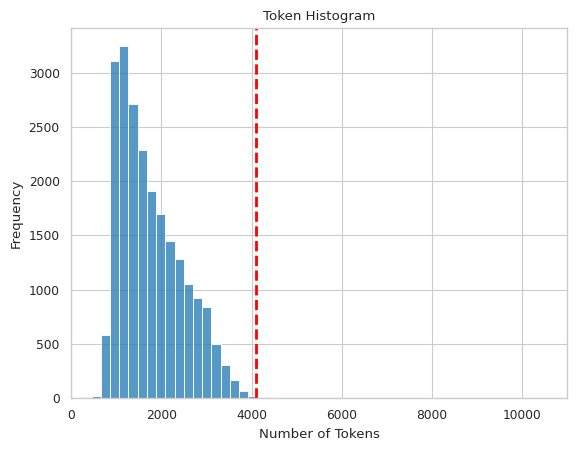
\includegraphics[width=\columnwidth]{token_distr.png}  % adjust as needed
  \caption{Distribution of token lengths of BillSum with max token indicator (BigBird PEGASUS).}
  \label{fig:token_distr}
\end{figure}

\indent We also perform EDA on the human-written summaries in the BillSum dataset to better understand the target output distribution and guide hyperparameter tuning for model training and generation. As shown in Table~\ref{tab:bill_len}, the average token length for a bill summary is 204, which is well within the generation capacity of models like PEGASUS and suitable for our compute constraints.

\indent Finally, we examine the average number of sentences per summary to inform our decisions regarding extractive techniques. Both cluster-based and MMR extraction methods require a hyperparameter specifying the number of sentences to include in the output. Based on our analysis, the average human-written summary in the BillSum dataset contains approximately 5.5 sentences. Accordingly, we set the output length for these extractive approaches to 6 sentences to align closely with the reference summaries.

\subsection{Evaluation Metrics}

To evaluate our generated summaries in comparison to human-written ones, we use ROUGE and BERTScore.\\

\noindent \textbf{ROUGE} is widely used for evaluating text summarization systems. It is simple and easy to interpret as it measures the lexical overlap between generated and reference summaries using n-grams and longest common subsequences. However, ROUGE is heavily surface-form dependent and may penalize valid paraphrases or semantically equivalent rewordings. Furthermore, it does not explicitly account for fluency or coherence.\\

\noindent \textbf{BERTScore} is a relatively newer metric for summarization that leverages contextual embeddings from BERT. It compares the semantic similarity between candidate and reference summaries at the token embedding level. This allows it to better capture paraphrasing and synonymy, making it a good candidate to balance our evaluation metrics. However, BERTScore is computationally more intensive and may be sensitive to the choice of the underlying language model.

\subsection{Baseline}

We use two extractive models as baselines to compare against our more advanced summarization approaches—cluster-based and MMR. For extractive summarization, the initial step involves segmenting the text into sentences or sentence-like units. We segment the bills based on the numbered section titles, followed by subsections labeled with lowercase letters, since conventional sentence splitting proves challenging due to the structured format of legal documents.\footnote{See Appendix Section~\ref{sec:appendix-a} for an example.} This approach provides a balance between segment length and information retention.

\indent We use Term Frequency–Inverse Document Frequency (TF-IDF) to vectorize each segmented unit for our extractive baselines. Despite its limitations in capturing semantic and contextual information \citep{9397119}, TF-IDF remains a common baseline due to its simplicity, interpretability, and low computational overhead.

\subsubsection{Cluster Extraction}

For cluster extraction, we use the sentence vectors generated by TF-IDF and perform clustering based on cosine distance. Guided by our EDA, we set the number of clusters to six, aligning with the average number of sentences in the human-written summaries. To extract a representative sentence from each cluster, we select the sentence whose vector is closest to the cluster centroid, capturing the most central content within that group.

\subsubsection{MMR Extraction}

Similar to cluster-based extraction, we utilize TF-IDF vectors for MMR and compute pairwise distances using cosine similarity. We designate the first sentence as the centroid for relevance scoring, motivated by the observation that the first sentence often contains the title or summary statement of the bill. As with the cluster-based extraction method, we fix the number of extracted sentences to six, aligning with the average length of human-written summaries in the BillSum dataset. The trade-off parameter $\lambda$ in the MMR scoring function is set to 0.7, prioritizing relevance to the document while still penalizing redundancy.

\subsection{Hybrid Models}

For our hybrid models, we build upon our existing extractive frameworks. This approach is motivated by our interest in directly measuring the performance improvements gained by incorporating abstractive techniques on top of extractive baselines. Additionally, many models have token limits and are computationally intensive. Shortening the input beforehand reduces compute time and information loss.

\subsubsection{Cluster + Longform Encoder-Decoder}

Our first hybrid model builds upon the key strengths on traditional extractive methods by integrating them with a few abstractive modeling techniques. The Cluster + LED model leverages the same initial extraction step, largely involving cluster-based sentence selection, to produce both concise and informative inputs tailored specifically for an abstractive summarization model like an LED.

We first applied a TF-IDF vectorization to segment legislative documents into sentence clusters, further selecting sentences that were more representative of each cluster using cosine similarity. We then fed the cluster-selected sentences into the LED model. LED in particular is well-suited for handling large inputs due to its sparse attention mechanism, efficiently identifying context and long range dependencies that may exist across large texts (perfect for summarization complex and well structured legal texts). 

\subsubsection{MMR + PEGASUS}

Our second hybrid model builds on the output of the MMR-based extractive summarization. The selected sentences are concatenated and fed into BigBird PEGASUS. We retain the same output length of six sentences, consistent with our extractive baselines. This choice enables the model to capture the key information needed for summarization while ensuring that inputs remain below the token limit, as illustrated in Figure~\ref{fig:token_distr_short}.

\begin{figure}[ht]
  \centering
  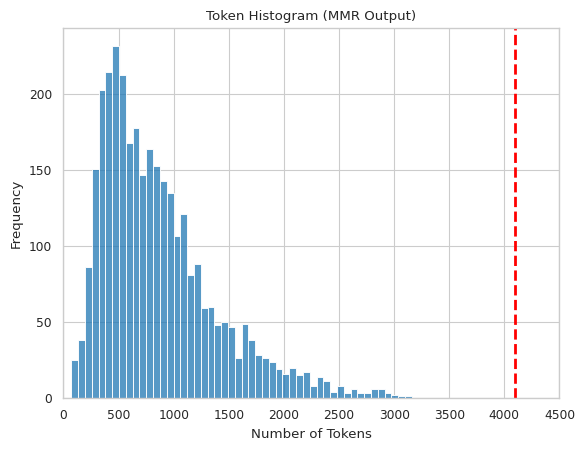
\includegraphics[width=\columnwidth]{token_distr_shortened.png}  % adjust as needed
  \caption{Distribution of token lengths of MMR output with max token indicator (BigBird PEGASUS).}
  \label{fig:token_distr_short}
\end{figure}

\subsection{BigBird PEGASUS}

BigBird PEGASUS is a transformer model that uses a sparse attention approach to improve performance on long texts over full attention transformers. While PEGASUS-large has a maximum input length of 1024 tokens, BigBird PEGASUS has a maximum input length of 4096 tokens, which is better suited to our bill summarization. PEGASUS would have only been able to fully process a small portion of the documents in BillSum, but BigBird PEGASUS is able to fully process almost all of them. 

Additionally, we performed fine-tuning on the model. BigBird PEGASUS was pretrained to summarize scientific papers from arxiv, which may have been slightly different to a legal document, so we evaluated the model's performance with the pretrained weights and after fine-tuning on BillSum. Due to time and computational resource constraints, we fine-tuned on a subset of 5000 bills from the training data for 1 epoch.

\section{Results and Discussion}

\begin{table*}[]
\centering
\begin{tabular}{l|llll|lll}
\multirow{2}{*}{\textbf{Model}} & \multicolumn{4}{c|}{\textbf{ROUGE}}                                          & \multicolumn{3}{c}{\textbf{BERTScore}}             \\ \cline{2-8} 
                                & \textbf{rouge-1} & \textbf{rouge-2} & \textbf{rouge-L} & \textbf{rouge-Lsum} & \textbf{Precision} & \textbf{Recall} & \textbf{F1} \\ \hline
Cluster                         & 0.3137           & 0.1725           & 0.2114           & 0.2772              & 0.7324             & 0.8399          & 0.7817      \\
MMR                             & 0.3117           & 0.1730           & 0.2010           & 0.2751              & 0.7367             & 0.8407          & 0.7845      \\
Cluster + LED                   & \textbf{0.4376}                 & \textbf{0.2629}                 &  \textbf{0.3229}                &  \textbf{0.3599}                   &  \textbf{0.8931}                  & \textbf{0.8659 }               & \textbf{0.8788}            \\
MMR + BigBird PEGASUS                   & 0.1759           & 0.0242           & 0.1169           & 0.1301              & 0.7981             & 0.7877          & 0.7924      \\
BigBird PEGASUS                  & 0.1931                 & 0.0253                 & 0.1259                 & 0.1419                    & 0.7907                   &  0.7893               &  0.7896          \\
Fine-Tuned BigBird PEGASUS                   & 0.2433                 &  0.0409                &  0.1534                & 0.1762                    & 0.8147                   &  0.8004               &  0.8072          
\end{tabular}
\caption{ROUGE and BERTScore results for proposed models.}
\label{tab:results}
\end{table*}

Looking at the results, we find that overall performance aligns with our expectations, with each model performing in line with its complexity and design—though a few unexpected outcomes also emerged.

\subsubsection{Baseline}

The Cluster and MMR extractive models had the lowest ROUGE/BERTScores and yielded nearly identical results, as shown in Table~\ref{tab:results}. We attribute this similarity to the dominant influence of sentence vectorization in these low-cost models, which likely limits the variance introduced by differing sentence selection strategies. In both models, we used TF-IDF for sentence vectorization, a frequency-based approach that is considered somewhat outdated compared to more context-aware embeddings. Using more up-to-date sentence embedding strategies, such as SentenceTransformers \citep{reimers-2019-sentence-bert}, may result in better performance and a more nuanced comparison.

\subsubsection{Hybrid Models}

For our hybrid models, we find that the evaluation results from our Cluster + LED model significantly outperformed both baseline and event abstractive methods in both ROUGE and BERTScore metrics. This indicates better semantic coherence with human-written summaries, along with preserving semantic relevance and generating human-like summaries, as shown in an F1 score of 0.8788. These findings largely highlight the effectiveness of hybrid summarization methods, particularly combining cluster-based extraction methodologies with perfect long-document parsers that the LED model can parse through. This combination addresses a lot of the unique challenges posed by long-form legal document summarization.

On the other hand, the MMR + BigBird PEGASUS model underperformed, achieving only a marginally higher F1 BERTScore compared to the extractive baseline (0.7924). We attribute this to the fixed output length of six sentences, which likely constrained the model’s ability to fully leverage its abstractive capabilities and synthesize broader contextual information from the input. However, it is important to note that the Cluster + LED model also operated under the same six-sentence constraint, yet still achieved noticeably better performance. This suggests that LED may be more efficient at leveraging limited input to generate coherent and informative summaries. Further experimentation could be helpful in determining the exact reasons for this difference.

\subsection{Abstractive Models}

The evaluation results for BigBird PEGASUS without fine-tuning show that the model performed very similarly the MMR + BigBird PEGASUS hybrid approach. This indicates that extractive approaches can provide an adequate approximation of the full text for the model to generate summaries of similar quality. The benefit of this is that the MMR text is significantly shorter than the full text, meaning the model is less resource intensive in generating summaries and can run faster.

Fine-tuning BigBird PEGASUS did noticeably improve all of the recorded metrics. As mentioned in the methods section, we only fine-tuned on a subset of 5000 records from the training data, which is about a quarter of the available data, for 1 epoch. Further research is required to determine how much performance would improve using the full training set and to determine the optimal number of training epochs. 

Both the base BigBird PEGASUS model and the fine-tuned model outperformed the baseline in precision and F1 BERTScore. However, both models performed worse than the baseline in recall BERTScore and all of the ROUGE metrics. This underperformance can be explained by how abstractive models generate summaries. Abstractive models do not copy text directly from the source like extractive models. Instead, they generate novel text using the source as a reference. This often results in summaries that are syntactically similar to the reference summaries, but may use different words to convey the same meaning. This results in a penalty on surface-form metrics like ROUGE. Similarly, BERTScore recall compares the embedding of each token in the reference to its most similar token in the candidate. The penalty BERTScore recall puts on abstractive generation is less severe than the penalty put on it by ROUGE metrics, but it can still be significant if the model significantly paraphrased the reference summary. BERTScore recall can also perform worse if the generated summaries are too short and do not cover everything the reference summaries cover.

\section{Conclusion}

We applied several extractive, abstractive, and hybrid approaches to generating summaries on the BillSum dataset. The results show that the hybrid and abstractive models can outperform the extractive models in semantics-based metrics like BERTScore, but can struggle with more surface-form metrics like ROUGE. We found that extractive methods can be used to create an approximation of the full text with a lower input token count, reducing the time and computational resources required to fine-tune and generate predictions with abstractive models without significantly impacting the quality of the generated summaries. Clustering in combination with LED in particular proved to be very effective at this task. Further research can test more combinations of extractive and abstractive models to create the best hybrid approach for long-form text. 

\section{Authors Contribution's}

Below we list the authors contributions for this paper (all authors contributed to the Methods/Results and Discussion sections):\\

\noindent Daniel: 

- Extractive Models (MMR, Cluster)\\
\indent- MMR + PEGASUS Hybrid Model\\
\indent- Introduction, Background, Slides (Introduction, Extractive) \\

\noindent Chris: 

- Hybrid Models (LED, LED + Cluster, Hyper-tuning)\\
\indent- LED + Cluster Hybrid Model\\
\indent- Abstract, Slides (Hybrid, Results)\\

\noindent Ryan: 

- Abstractive Models (BigBird PEGASUS)\\
\indent- Conclusion, Slides (Abstractive, Conclusion)\\

\nocite{Eidelman_2019, agarwal-etal-2022-extractive, 9397119, Jain2024-ht, pmlr-v119-zhang20ae, zaheer2021bigbirdtransformerslonger, reimers-2019-sentence-bert}



% Entries for the entire Anthology, followed by custom entries
\bibliography{anthology,custom}
\bibliographystyle{acl_natbib}

\appendix

\section{BillSum Bill Structure}
\label{sec:appendix-a}
\begin{figure}[ht]
  \centering
  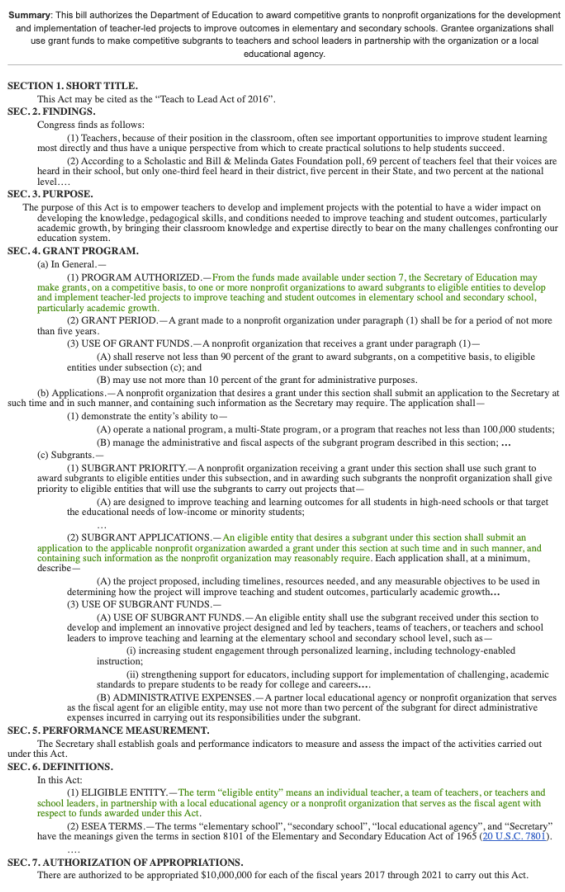
\includegraphics[width=\columnwidth]{US_bill.png}  % adjust as needed
  \caption{An example Congressional bill, from the BillSum paper.}
  \label{fig:congressional_bill}
\end{figure}

\end{document}
